% Options for packages loaded elsewhere
% Options for packages loaded elsewhere
\PassOptionsToPackage{unicode}{hyperref}
\PassOptionsToPackage{hyphens}{url}
\PassOptionsToPackage{dvipsnames,svgnames,x11names}{xcolor}
%
\documentclass[
  ngerman,
  letterpaper,
  DIV=11]{scrartcl}
\usepackage{xcolor}
\usepackage{amsmath,amssymb}
\setcounter{secnumdepth}{5}
\usepackage{iftex}
\ifPDFTeX
  \usepackage[T1]{fontenc}
  \usepackage[utf8]{inputenc}
  \usepackage{textcomp} % provide euro and other symbols
\else % if luatex or xetex
  \usepackage{unicode-math} % this also loads fontspec
  \defaultfontfeatures{Scale=MatchLowercase}
  \defaultfontfeatures[\rmfamily]{Ligatures=TeX,Scale=1}
\fi
\usepackage{lmodern}
\ifPDFTeX\else
  % xetex/luatex font selection
\fi
% Use upquote if available, for straight quotes in verbatim environments
\IfFileExists{upquote.sty}{\usepackage{upquote}}{}
\IfFileExists{microtype.sty}{% use microtype if available
  \usepackage[]{microtype}
  \UseMicrotypeSet[protrusion]{basicmath} % disable protrusion for tt fonts
}{}
\makeatletter
\@ifundefined{KOMAClassName}{% if non-KOMA class
  \IfFileExists{parskip.sty}{%
    \usepackage{parskip}
  }{% else
    \setlength{\parindent}{0pt}
    \setlength{\parskip}{6pt plus 2pt minus 1pt}}
}{% if KOMA class
  \KOMAoptions{parskip=half}}
\makeatother
% Make \paragraph and \subparagraph free-standing
\makeatletter
\ifx\paragraph\undefined\else
  \let\oldparagraph\paragraph
  \renewcommand{\paragraph}{
    \@ifstar
      \xxxParagraphStar
      \xxxParagraphNoStar
  }
  \newcommand{\xxxParagraphStar}[1]{\oldparagraph*{#1}\mbox{}}
  \newcommand{\xxxParagraphNoStar}[1]{\oldparagraph{#1}\mbox{}}
\fi
\ifx\subparagraph\undefined\else
  \let\oldsubparagraph\subparagraph
  \renewcommand{\subparagraph}{
    \@ifstar
      \xxxSubParagraphStar
      \xxxSubParagraphNoStar
  }
  \newcommand{\xxxSubParagraphStar}[1]{\oldsubparagraph*{#1}\mbox{}}
  \newcommand{\xxxSubParagraphNoStar}[1]{\oldsubparagraph{#1}\mbox{}}
\fi
\makeatother

\usepackage{color}
\usepackage{fancyvrb}
\newcommand{\VerbBar}{|}
\newcommand{\VERB}{\Verb[commandchars=\\\{\}]}
\DefineVerbatimEnvironment{Highlighting}{Verbatim}{commandchars=\\\{\}}
% Add ',fontsize=\small' for more characters per line
\usepackage{framed}
\definecolor{shadecolor}{RGB}{241,243,245}
\newenvironment{Shaded}{\begin{snugshade}}{\end{snugshade}}
\newcommand{\AlertTok}[1]{\textcolor[rgb]{0.68,0.00,0.00}{#1}}
\newcommand{\AnnotationTok}[1]{\textcolor[rgb]{0.37,0.37,0.37}{#1}}
\newcommand{\AttributeTok}[1]{\textcolor[rgb]{0.40,0.45,0.13}{#1}}
\newcommand{\BaseNTok}[1]{\textcolor[rgb]{0.68,0.00,0.00}{#1}}
\newcommand{\BuiltInTok}[1]{\textcolor[rgb]{0.00,0.23,0.31}{#1}}
\newcommand{\CharTok}[1]{\textcolor[rgb]{0.13,0.47,0.30}{#1}}
\newcommand{\CommentTok}[1]{\textcolor[rgb]{0.37,0.37,0.37}{#1}}
\newcommand{\CommentVarTok}[1]{\textcolor[rgb]{0.37,0.37,0.37}{\textit{#1}}}
\newcommand{\ConstantTok}[1]{\textcolor[rgb]{0.56,0.35,0.01}{#1}}
\newcommand{\ControlFlowTok}[1]{\textcolor[rgb]{0.00,0.23,0.31}{\textbf{#1}}}
\newcommand{\DataTypeTok}[1]{\textcolor[rgb]{0.68,0.00,0.00}{#1}}
\newcommand{\DecValTok}[1]{\textcolor[rgb]{0.68,0.00,0.00}{#1}}
\newcommand{\DocumentationTok}[1]{\textcolor[rgb]{0.37,0.37,0.37}{\textit{#1}}}
\newcommand{\ErrorTok}[1]{\textcolor[rgb]{0.68,0.00,0.00}{#1}}
\newcommand{\ExtensionTok}[1]{\textcolor[rgb]{0.00,0.23,0.31}{#1}}
\newcommand{\FloatTok}[1]{\textcolor[rgb]{0.68,0.00,0.00}{#1}}
\newcommand{\FunctionTok}[1]{\textcolor[rgb]{0.28,0.35,0.67}{#1}}
\newcommand{\ImportTok}[1]{\textcolor[rgb]{0.00,0.46,0.62}{#1}}
\newcommand{\InformationTok}[1]{\textcolor[rgb]{0.37,0.37,0.37}{#1}}
\newcommand{\KeywordTok}[1]{\textcolor[rgb]{0.00,0.23,0.31}{\textbf{#1}}}
\newcommand{\NormalTok}[1]{\textcolor[rgb]{0.00,0.23,0.31}{#1}}
\newcommand{\OperatorTok}[1]{\textcolor[rgb]{0.37,0.37,0.37}{#1}}
\newcommand{\OtherTok}[1]{\textcolor[rgb]{0.00,0.23,0.31}{#1}}
\newcommand{\PreprocessorTok}[1]{\textcolor[rgb]{0.68,0.00,0.00}{#1}}
\newcommand{\RegionMarkerTok}[1]{\textcolor[rgb]{0.00,0.23,0.31}{#1}}
\newcommand{\SpecialCharTok}[1]{\textcolor[rgb]{0.37,0.37,0.37}{#1}}
\newcommand{\SpecialStringTok}[1]{\textcolor[rgb]{0.13,0.47,0.30}{#1}}
\newcommand{\StringTok}[1]{\textcolor[rgb]{0.13,0.47,0.30}{#1}}
\newcommand{\VariableTok}[1]{\textcolor[rgb]{0.07,0.07,0.07}{#1}}
\newcommand{\VerbatimStringTok}[1]{\textcolor[rgb]{0.13,0.47,0.30}{#1}}
\newcommand{\WarningTok}[1]{\textcolor[rgb]{0.37,0.37,0.37}{\textit{#1}}}

\usepackage{longtable,booktabs,array}
\usepackage{calc} % for calculating minipage widths
% Correct order of tables after \paragraph or \subparagraph
\usepackage{etoolbox}
\makeatletter
\patchcmd\longtable{\par}{\if@noskipsec\mbox{}\fi\par}{}{}
\makeatother
% Allow footnotes in longtable head/foot
\IfFileExists{footnotehyper.sty}{\usepackage{footnotehyper}}{\usepackage{footnote}}
\makesavenoteenv{longtable}
\usepackage{graphicx}
\makeatletter
\newsavebox\pandoc@box
\newcommand*\pandocbounded[1]{% scales image to fit in text height/width
  \sbox\pandoc@box{#1}%
  \Gscale@div\@tempa{\textheight}{\dimexpr\ht\pandoc@box+\dp\pandoc@box\relax}%
  \Gscale@div\@tempb{\linewidth}{\wd\pandoc@box}%
  \ifdim\@tempb\p@<\@tempa\p@\let\@tempa\@tempb\fi% select the smaller of both
  \ifdim\@tempa\p@<\p@\scalebox{\@tempa}{\usebox\pandoc@box}%
  \else\usebox{\pandoc@box}%
  \fi%
}
% Set default figure placement to htbp
\def\fps@figure{htbp}
\makeatother



\ifLuaTeX
\usepackage[bidi=basic]{babel}
\else
\usepackage[bidi=default]{babel}
\fi
% get rid of language-specific shorthands (see #6817):
\let\LanguageShortHands\languageshorthands
\def\languageshorthands#1{}
\ifLuaTeX
  \usepackage[german]{selnolig} % disable illegal ligatures
\fi


\setlength{\emergencystretch}{3em} % prevent overfull lines

\providecommand{\tightlist}{%
  \setlength{\itemsep}{0pt}\setlength{\parskip}{0pt}}



 


\KOMAoption{captions}{tableheading}
\makeatletter
\@ifpackageloaded{caption}{}{\usepackage{caption}}
\AtBeginDocument{%
\ifdefined\contentsname
  \renewcommand*\contentsname{Inhaltsverzeichnis}
\else
  \newcommand\contentsname{Inhaltsverzeichnis}
\fi
\ifdefined\listfigurename
  \renewcommand*\listfigurename{Abbildungsverzeichnis}
\else
  \newcommand\listfigurename{Abbildungsverzeichnis}
\fi
\ifdefined\listtablename
  \renewcommand*\listtablename{Tabellenverzeichnis}
\else
  \newcommand\listtablename{Tabellenverzeichnis}
\fi
\ifdefined\figurename
  \renewcommand*\figurename{Abbildung}
\else
  \newcommand\figurename{Abbildung}
\fi
\ifdefined\tablename
  \renewcommand*\tablename{Tabelle}
\else
  \newcommand\tablename{Tabelle}
\fi
}
\@ifpackageloaded{float}{}{\usepackage{float}}
\floatstyle{ruled}
\@ifundefined{c@chapter}{\newfloat{codelisting}{h}{lop}}{\newfloat{codelisting}{h}{lop}[chapter]}
\floatname{codelisting}{Listing}
\newcommand*\listoflistings{\listof{codelisting}{Listingverzeichnis}}
\makeatother
\makeatletter
\makeatother
\makeatletter
\@ifpackageloaded{caption}{}{\usepackage{caption}}
\@ifpackageloaded{subcaption}{}{\usepackage{subcaption}}
\makeatother
\usepackage{bookmark}
\IfFileExists{xurl.sty}{\usepackage{xurl}}{} % add URL line breaks if available
\urlstyle{same}
\hypersetup{
  pdftitle={De ingenio non est disputandum},
  pdfauthor={N.N.},
  pdflang={de},
  colorlinks=true,
  linkcolor={blue},
  filecolor={Maroon},
  citecolor={Blue},
  urlcolor={Blue},
  pdfcreator={LaTeX via pandoc}}


\title{De ingenio non est disputandum}
\usepackage{etoolbox}
\makeatletter
\providecommand{\subtitle}[1]{% add subtitle to \maketitle
  \apptocmd{\@title}{\par {\large #1 \par}}{}{}
}
\makeatother
\subtitle{Intertemporale Optimierung der KI-Nutzung: Warum kognitive
Assistenzsysteme nicht alle zu Junkies oder Genies machen}
\author{Jan S. Voßwinkel}
\date{today}
\begin{document}
\maketitle

\renewcommand*\contentsname{Inhaltsverzeichnis}
{
\hypersetup{linkcolor=}
\setcounter{tocdepth}{3}
\tableofcontents
}

\subsection{Einleitung: Das E-Bike-Paradoxon der kognitiven
Arbeit}\label{einleitung-das-e-bike-paradoxon-der-kognitiven-arbeit}

Die rasante Verbreitung generativer Künstlicher Intelligenz (KI) in der
Hochschulbildung steht im Zentrum einer polarisierten Debatte. Während
die eine Seite KI als unerschöpflichen Produktivitätsbooster feiert, der
Lernende von kognitiver Routinearbeit befreit, warnt die andere Seite
vor digitaler Demenz und intellektueller Atrophie.

In Anlehnung an den klassischen Aufsatz von Stigler und Becker (1977),
\emph{„De gustibus non est disputandum``}, argumentiert dieser Beitrag:
\textbf{De ingenio non est disputandum}. Die Effekte der KI auf das
kognitive Kapital der Studierenden sind keine Frage unveränderlicher,
exogener Begabungen oder fatalistischer Technologiefolgen. Vielmehr sind
sie das Resultat rationaler, intertemporaler Allokationsentscheidungen
im Kontext spezifischer Anreizstrukturen.

Um diese Dynamik greifbar zu machen, bietet sich die \textbf{Analogie
des E-Bikes} an: Der Elektromotor (analog zur KI) ist konstruiert, um
die eigene Tretleistung zu unterstützen, insbesondere am Berg.

\begin{itemize}
\tightlist
\item
  \textbf{Der Synergie-Pfad (Komplementäre Nutzung):} Ein Fahrer nutzt
  die motorische Unterstützung, um längere, anspruchsvollere Strecken zu
  bewältigen, die er zuvor gemieden hätte. Weil er die Pedale weiterhin
  intensiv bedient, baut er -- trotz (oder gerade wegen) des Motors --
  mehr Kondition und Muskelmasse auf.
\item
  \textbf{Der Substitutions-Pfad (Das E-Bike als Moped):} Ein anderer
  Fahrer nutzt die volle Motorleistung, um jegliche eigene
  Tretanstrengung zu vermeiden. Er erreicht sein Ziel zwar ebenso
  schnell und mühelos, verliert jedoch über die Zeit drastisch an
  muskulärer und kardiovaskulärer Fitness.
\end{itemize}

Dieses Paper formalisiert diese Intuition in einem mikroökonomischen
Multi-Perioden-Modell. Durch den Verzicht auf die komplexe
Bellman-Gleichung und den Einsatz des klassischen Euler-Kalküls der
lokalen Variation zeigen wir: Ob KI als kognitiver Multiplikator oder
als intellektuelle Atrophie-Falle wirkt, hängt exakt davon ab, ob die
eigene Anstrengung eine kritische Schwelle überschreitet.

\begin{center}\rule{0.5\linewidth}{0.5pt}\end{center}

\subsection{Das Modell: Zeitbudget, Produktion und
Kapitalakkumulation}\label{das-modell-zeitbudget-produktion-und-kapitalakkumulation}

Wir betrachten einen rationalen Studierenden, der seinen Nutzen über
einen Studienverlauf von \(T\) Perioden maximiert.

\subsubsection{Zeitbudget und Freizeit}\label{zeitbudget-und-freizeit}

In jeder Periode \(t\) verfügt der Studierende über ein exogenes
Zeitbudget \(\bar{T}\), das er auf eigene kognitive Anstrengung \(E_t\)
(z. B. tiefes Denken, Problemlösen, Prompt-Design) und Freizeit \(F_t\)
aufteilt. Der Einfachheit halber nehmen wir an, dass die rein technische
Nutzung der KI \(A_t\) kurzfristig als perfektes Substitut zur eigenen
Leistung fungiert und keine nennenswerte eigene Zeit beansprucht. Die
Freizeit ergibt sich somit als:

\[F_t = \bar{T} - E_t\]

\subsubsection{Die akademische
Produktionsfunktion}\label{die-akademische-produktionsfunktion}

Der sichtbare akademische Output \(Y_t\) (z. B. Noten, abgegebene
Hausarbeiten, Präsentationen) in Periode \(t\) wird durch eine lineare
Produktionsfunktion bestimmt. Diese kombiniert das bestehende kognitive
Basiswissen \(K_t\), die eigene Anstrengung \(E_t\) und den Umfang der
KI-Nutzung \(A_t\):

\[Y_t = (K_t \cdot E_t) + A_t\]

\subsubsection{Akkumulation des kognitiven Kapitals (Die
„Muskel-Gleichung``)}\label{akkumulation-des-kognitiven-kapitals-die-muskel-gleichung}

Das Bindeglied zwischen den Perioden ist die Veränderung des
Wissensbestandes \(K_t\). Wissen entsteht durch eigene Anstrengung
(\(\alpha\)), verfällt mit der natürlichen Vergessensrate
\(\delta \in (0, 1)\) und wird durch die KI entweder synergetisch
verstärkt (\(\beta\)) oder durch Substitution erodiert (\(\gamma\)):

\[K_{t+1} = (1 - \delta) K_t + \alpha E_t + \beta (E_t \cdot A_t) - \gamma A_t\]

Die partielle Ableitung der Akkumulationsgleichung nach dem KI-Konsum
liefert die \textbf{Netto-Atrophie} des Systems:

\[\frac{\partial K_{t+1}}{\partial A_t} = \beta E_t - \gamma = -(\gamma - \beta E_t)\]

Aus diesem Term lässt sich eine \textbf{kritische Anstrengungsschwelle}
\(E^*\) ableiten:

\[E^* = \frac{\gamma}{\beta}\]

\begin{itemize}
\tightlist
\item
  \textbf{Komplementarität (\(E_t > E^*\)):} Investiert der Studierende
  hohe eigene Tretleistung, überwiegt der Synergie-Effekt
  (\(\beta E_t > \gamma\)). Die KI wirkt wie der E-Bike-Motor im
  Sport-Modus: Sie ermöglicht ein tieferes Durchdringen des Stoffs; das
  kognitive Kapital wächst.
\item
  \textbf{Substitution (\(E_t < E^*\)):} Bei geringer Eigenanstrengung
  überwiegt die Atrophie (\(\gamma > \beta E_t\)). Die KI ersetzt das
  eigene Denken; der kognitive Kapitalstock verfällt.
\end{itemize}

\begin{center}\rule{0.5\linewidth}{0.5pt}\end{center}

\subsection{Intertemporale Optimierung: Der
Euler-Kalkül}\label{intertemporale-optimierung-der-euler-kalkuxfcl}

\subsubsection{Die
Cobb-Douglas-Nutzenfunktion}\label{die-cobb-douglas-nutzenfunktion}

Der Nutzen in Periode \(t\) wird durch eine Cobb-Douglas-Funktion
abgebildet, die den Erfolg im Studium (\(Y_t\)) und den Genuss von
Freizeit (\(F_t\)) mit den Elastizitäten \(\mu \in (0, 1)\) und
\((1-\mu)\) gewichtet:

\[U(Y_t, F_t) = Y_t^\mu \cdot (\bar{T} - E_t)^{1-\mu}\]

Diese Spezifikation ist aus zwei Gründen zentral: 1. \textbf{Abnehmender
Grenznutzen im Output:} Da
\(\frac{\partial U_t}{\partial Y_t} = \mu \frac{U_t}{Y_t}\) gilt, sinkt
der marginale Nutzen zusätzlichen Outputs, je höher \(Y_t\) bereits ist.
Ein Studierender hat kein Interesse an einer unendlichen Ausdehnung von
\(Y_t\), da eine Zeugnisnote von „1,0`` nicht weiter verbessert werden
kann. 2. \textbf{Endogene Sättigung (\(K_{\max}\) und \(A_{\max}\)):}
Weil die eigene Anstrengung \(E_t\) durch das Zeitbudget \(\bar{T}\) und
das Bedürfnis nach Freizeit nach oben gedeckelt ist, können die
Wissenszuwächse nicht unendlich steigen. Es existiert ein langfristiger
Steady State (\(K_{\max}\)), an dem die natürliche Vergessensrate
\(\delta K_t\) exakt der Neuinvestition entspricht.

\subsubsection{Die intertemporale
Euler-Gleichung}\label{die-intertemporale-euler-gleichung}

Statt das Problem über eine rekursive Bellman-Gleichung zu lösen, nutzen
wir das methodisch elegante Prinzip der \textbf{lokalen Variation}
(Euler-Kalkül).

\begin{quote}
\textbf{Methodischer Hinweis zum Multi-Perioden-Fall:} Wenn ein Zeitpfad
über \(T\) Perioden optimal ist, muss er auch zwischen jeweils zwei
direkt aufeinanderfolgenden Perioden \(t\) und \(t+1\) optimal sein. Wir
betrachten eine marginale Erhöhung der KI-Dosis in Periode \(t\), die
wir durch eine Gegenanpassung in Periode \(t+1\) so kompensieren, dass
der Kapitalstock in Periode \(t+2\) völlig unverändert bleibt. Die
Optimierungsbedingung zwischen \(t\) und \(t+1\) gilt somit fundamental
für jede Periode im gesamten Studienverlauf.
\end{quote}

Das intertemporale Gleichgewicht verlangt, dass der marginale
Nutzenzugewinn einer Ausdehnung von \(A_t\) heute exakt dem
diskontierten Nutzenverlust durch den veränderten Kapitalstock morgen
entspricht (\(\rho \in (0,1)\) bezeichnet den Diskontierungsfaktor):

\[\underbrace{\frac{\partial U(Y_t)}{\partial Y_t} \cdot \frac{\partial Y_t}{\partial A_t}}_{\substack{\text{Kurzfristiger Grenzgewinn heute} \\ \text{(Sofortige Entlastung / Output-Plus)}}} = \underbrace{\rho \cdot \left( \frac{\partial U(Y_{t+1})}{\partial Y_{t+1}} \cdot \frac{\partial Y_{t+1}}{\partial K_{t+1}} \right)}_{\substack{\text{Diskontierter Grenz-Wert} \\ \text{des Wissens morgen}}} \cdot \underbrace{(\gamma - \beta E_t)}_{\substack{\text{Netto-Atrophie} \\ \text{(Marginaler Wissensverlust)}}}\]

Mit den Ableitungen unseres Modells
(\(\frac{\partial Y_t}{\partial A_t} = 1\),
\(\frac{\partial Y_{t+1}}{\partial K_{t+1}} = E_{t+1}\) und der
Cobb-Douglas-Elastizität) vereinfacht sich die \textbf{Euler-Gleichung
für den optimalen KI-Konsum} zu:

\[\underbrace{\mu \frac{U_t}{Y_t}}_{\text{Grenznutzen heute}} = \underbrace{\rho \cdot \mu \frac{U_{t+1}}{Y_{t+1}} \cdot E_{t+1}}_{\text{Schattenpreis des Wissens}} \cdot \underbrace{(\gamma - \beta E_t)}_{\text{Netto-Atrophie}}\]

\begin{center}\rule{0.5\linewidth}{0.5pt}\end{center}

\subsection{Zwei Pfade der KI-Nutzung: Simulation und
Dynamik}\label{zwei-pfade-der-ki-nutzung-simulation-und-dynamik}

Die Euler-Gleichung erklärt formal, warum sich im Studienverlauf zwei
diametral entgegengesetzte Nutzungsweisen und Karrieren ausbilden:

\subsubsection{Der Synergie-Pfad (Das E-Bike im
Sport-Modus)}\label{der-synergie-pfad-das-e-bike-im-sport-modus}

Wählt ein Studierender eine hohe Eigenanstrengung (\(E > E^*\)), wird
der Term \((\gamma - \beta E)\) negativ. Die intertemporalen Kosten der
KI verwandeln sich in eine \textbf{kognitive Rendite}. Der
Wissensbestand \(K_t\) steigt an. Weil sein Output \(Y_t\) durch das
hohe Wissen wächst, greift der abnehmende Grenznutzen der
Cobb-Douglas-Funktion: Der Studierende nutzt die KI hochprofessionell
als Werkzeug, stabilisiert seinen Konsum jedoch auf einem gesunden
Niveau (\(A_{\max}\)), um seine Freizeit zu genießen.

\subsubsection{Der Substitutions-Pfad (Die
Kompensations-Spirale)}\label{der-substitutions-pfad-die-kompensations-spirale}

Wählt ein Studierender eine geringe Eigenanstrengung (\(E < E^*\)), ist
die Netto-Atrophie positiv. Das Wissen \(K_t\) erodiert. In der Folge
droht der Output \(Y_t\) abzusacken, was den Grenznutzen
\(\mu \frac{U}{Y}\) explodieren ließe (Notenabsturz). Um die
Euler-Gleichung im Gleichgewicht zu halten und das Satisficing-Ziel zu
sichern, \textbf{muss} der Studierende seinen KI-Konsum \(A_t\)
kontinuierlich erhöhen. Er gerät in eine Abhängigkeitsspirale: Er nutzt
mehr KI, nicht weil er produktiver wird, sondern um seinen endogenen
Wissensverfall zu kompensieren.

\begin{center}\rule{0.5\linewidth}{0.5pt}\end{center}

\subsection{Grafische Simulation in R}\label{grafische-simulation-in-r}

Die folgende Simulation operationalisiert das Gesamtmodell für 25
Semesterwochen und stellt die beiden Pfade im direkten Vergleich dar.

\begin{Shaded}
\begin{Highlighting}[]
\FunctionTok{library}\NormalTok{(tidyverse)}

\CommentTok{\# 1. Modellparameter}
\FunctionTok{set.seed}\NormalTok{(}\DecValTok{2026}\NormalTok{)}
\NormalTok{t\_max }\OtherTok{\textless{}{-}} \DecValTok{25}          \CommentTok{\# Betrachtungszeitraum (Semesterwochen)}
\NormalTok{bar\_T }\OtherTok{\textless{}{-}} \DecValTok{40}          \CommentTok{\# Zeitbudget pro Woche (Wochenstunden)}
\NormalTok{K\_0 }\OtherTok{\textless{}{-}} \DecValTok{10}            \CommentTok{\# Initiales kognitives Basiswissen}
\NormalTok{delta }\OtherTok{\textless{}{-}} \FloatTok{0.08}        \CommentTok{\# Natürliche Vergessensrate (8\%)}
\NormalTok{alpha }\OtherTok{\textless{}{-}} \FloatTok{0.4}         \CommentTok{\# Lerneffizienz durch Eigenanstrengung}
\NormalTok{beta }\OtherTok{\textless{}{-}} \FloatTok{0.05}         \CommentTok{\# Synergie{-}Parameter (Komplementarität)}
\NormalTok{gamma }\OtherTok{\textless{}{-}} \FloatTok{0.20}        \CommentTok{\# Atrophie{-}Parameter (Substitution)}

\CommentTok{\# Kritische Anstrengungsschwelle E* = gamma / beta = 0.20 / 0.05 = 4 Stunden}
\NormalTok{E\_A }\OtherTok{\textless{}{-}} \DecValTok{8}             \CommentTok{\# Student A: Sport{-}Modus (E = 8 Std. \textgreater{} E* {-}\textgreater{} 32 Std. Freizeit)}
\NormalTok{E\_B }\OtherTok{\textless{}{-}} \DecValTok{2}             \CommentTok{\# Student B: Moped{-}Modus (E = 2 Std. \textless{} E* {-}\textgreater{} 38 Std. Freizeit)}

\CommentTok{\# Nutzenparameter}
\NormalTok{mu }\OtherTok{\textless{}{-}} \FloatTok{0.5}            \CommentTok{\# Cobb{-}Douglas Gewichtung (50\% Output, 50\% Freizeit)}

\CommentTok{\# Verhaltensparameter abgeleitet aus Euler \& Cobb{-}Douglas{-}Sättigung:}
\NormalTok{tau }\OtherTok{\textless{}{-}} \FloatTok{0.3}           \CommentTok{\# Absorptive Kapazität für sinnvolle KI{-}Nutzung (Student A)}
\NormalTok{Y\_ziel\_B }\OtherTok{\textless{}{-}} \DecValTok{25}       \CommentTok{\# Satisficing{-}Output{-}Ziel gegen Zeugnisabsturz (Student B)}

\CommentTok{\# 2. Datenspeicher initialisieren}
\NormalTok{time }\OtherTok{\textless{}{-}} \DecValTok{1}\SpecialCharTok{:}\NormalTok{t\_max}
\NormalTok{K\_A }\OtherTok{\textless{}{-}} \FunctionTok{numeric}\NormalTok{(t\_max); K\_A[}\DecValTok{1}\NormalTok{] }\OtherTok{\textless{}{-}}\NormalTok{ K\_0; Y\_A }\OtherTok{\textless{}{-}} \FunctionTok{numeric}\NormalTok{(t\_max); A\_A }\OtherTok{\textless{}{-}} \FunctionTok{numeric}\NormalTok{(t\_max); U\_A }\OtherTok{\textless{}{-}} \FunctionTok{numeric}\NormalTok{(t\_max)}
\NormalTok{K\_B }\OtherTok{\textless{}{-}} \FunctionTok{numeric}\NormalTok{(t\_max); K\_B[}\DecValTok{1}\NormalTok{] }\OtherTok{\textless{}{-}}\NormalTok{ K\_0; Y\_B }\OtherTok{\textless{}{-}} \FunctionTok{numeric}\NormalTok{(t\_max); A\_B }\OtherTok{\textless{}{-}} \FunctionTok{numeric}\NormalTok{(t\_max); U\_B }\OtherTok{\textless{}{-}} \FunctionTok{numeric}\NormalTok{(t\_max)}

\CommentTok{\# 3. Simulation über den Zeitverlauf}
\ControlFlowTok{for}\NormalTok{ (t }\ControlFlowTok{in} \DecValTok{1}\SpecialCharTok{:}\NormalTok{t\_max) \{}
  
  \CommentTok{\# {-}{-}{-} PFAD A: SYNERGIE (Sport{-}Modus) {-}{-}{-}}
  \CommentTok{\# KI wächst mit Wissen, flacht aber asymptotisch ab (abnehmender Grenznutzen)}
\NormalTok{  A\_A[t] }\OtherTok{\textless{}{-}}\NormalTok{ tau }\SpecialCharTok{*}\NormalTok{ K\_A[t]}
\NormalTok{  Y\_A[t] }\OtherTok{\textless{}{-}}\NormalTok{ (K\_A[t] }\SpecialCharTok{*}\NormalTok{ E\_A) }\SpecialCharTok{+}\NormalTok{ A\_A[t]                          }
\NormalTok{  U\_A[t] }\OtherTok{\textless{}{-}}\NormalTok{ (Y\_A[t]}\SpecialCharTok{\^{}}\NormalTok{mu) }\SpecialCharTok{*}\NormalTok{ ((bar\_T }\SpecialCharTok{{-}}\NormalTok{ E\_A)}\SpecialCharTok{\^{}}\NormalTok{(}\DecValTok{1} \SpecialCharTok{{-}}\NormalTok{ mu))           }
  
  \ControlFlowTok{if}\NormalTok{ (t }\SpecialCharTok{\textless{}}\NormalTok{ t\_max) \{}
\NormalTok{    K\_A[t}\SpecialCharTok{+}\DecValTok{1}\NormalTok{] }\OtherTok{\textless{}{-}}\NormalTok{ (}\DecValTok{1} \SpecialCharTok{{-}}\NormalTok{ delta) }\SpecialCharTok{*}\NormalTok{ K\_A[t] }\SpecialCharTok{+}\NormalTok{ alpha }\SpecialCharTok{*}\NormalTok{ E\_A }\SpecialCharTok{+}\NormalTok{ beta }\SpecialCharTok{*}\NormalTok{ (E\_A }\SpecialCharTok{*}\NormalTok{ A\_A[t]) }\SpecialCharTok{{-}}\NormalTok{ gamma }\SpecialCharTok{*}\NormalTok{ A\_A[t]}
\NormalTok{  \}}
  
  \CommentTok{\# {-}{-}{-} PFAD B: SUBSTITUTION (Moped{-}Modus) {-}{-}{-}}
  \CommentTok{\# KI muss steigen, um Wissensverfall (K {-}\textgreater{} 0) zu kompensieren}
\NormalTok{  A\_B[t] }\OtherTok{\textless{}{-}} \FunctionTok{max}\NormalTok{(}\DecValTok{0}\NormalTok{, Y\_ziel\_B }\SpecialCharTok{{-}}\NormalTok{ (K\_B[t] }\SpecialCharTok{*}\NormalTok{ E\_B))}
\NormalTok{  Y\_B[t] }\OtherTok{\textless{}{-}}\NormalTok{ (K\_B[t] }\SpecialCharTok{*}\NormalTok{ E\_B) }\SpecialCharTok{+}\NormalTok{ A\_B[t]                          }
\NormalTok{  U\_B[t] }\OtherTok{\textless{}{-}}\NormalTok{ (Y\_B[t]}\SpecialCharTok{\^{}}\NormalTok{mu) }\SpecialCharTok{*}\NormalTok{ ((bar\_T }\SpecialCharTok{{-}}\NormalTok{ E\_B)}\SpecialCharTok{\^{}}\NormalTok{(}\DecValTok{1} \SpecialCharTok{{-}}\NormalTok{ mu))           }
  
  \ControlFlowTok{if}\NormalTok{ (t }\SpecialCharTok{\textless{}}\NormalTok{ t\_max) \{}
\NormalTok{    K\_B[t}\SpecialCharTok{+}\DecValTok{1}\NormalTok{] }\OtherTok{\textless{}{-}} \FunctionTok{max}\NormalTok{(}\FloatTok{0.5}\NormalTok{, (}\DecValTok{1} \SpecialCharTok{{-}}\NormalTok{ delta) }\SpecialCharTok{*}\NormalTok{ K\_B[t] }\SpecialCharTok{+}\NormalTok{ alpha }\SpecialCharTok{*}\NormalTok{ E\_B }\SpecialCharTok{+}\NormalTok{ beta }\SpecialCharTok{*}\NormalTok{ (E\_B }\SpecialCharTok{*}\NormalTok{ A\_B[t]) }\SpecialCharTok{{-}}\NormalTok{ gamma }\SpecialCharTok{*}\NormalTok{ A\_B[t])}
\NormalTok{  \}}
\NormalTok{\}}

\CommentTok{\# 4. Datenaufbereitung im Tidy{-}Format}
\NormalTok{df\_sim }\OtherTok{\textless{}{-}} \FunctionTok{tibble}\NormalTok{(}
  \AttributeTok{Zeit =} \FunctionTok{rep}\NormalTok{(time, }\DecValTok{2}\NormalTok{),}
  \AttributeTok{Student =} \FunctionTok{rep}\NormalTok{(}\FunctionTok{c}\NormalTok{(}\StringTok{"Synergie{-}Pfad (E = 8 Std. \textgreater{} E*: Wissensaufbau \& Sättigung)"}\NormalTok{, }
                  \StringTok{"Substitutions{-}Pfad (E = 2 Std. \textless{} E*: Wissensverfall \& Kompensation)"}\NormalTok{), }\AttributeTok{each =}\NormalTok{ t\_max),}
  \AttributeTok{Kognitives\_Kapital =} \FunctionTok{c}\NormalTok{(K\_A, K\_B),}
  \AttributeTok{KI\_Dosis =} \FunctionTok{c}\NormalTok{(A\_A, A\_B),}
  \AttributeTok{Output =} \FunctionTok{c}\NormalTok{(Y\_A, Y\_B),}
  \AttributeTok{Nutzen =} \FunctionTok{c}\NormalTok{(U\_A, U\_B)}
\NormalTok{) }\SpecialCharTok{\%\textgreater{}\%}
  \FunctionTok{pivot\_longer}\NormalTok{(}\AttributeTok{cols =} \FunctionTok{c}\NormalTok{(Kognitives\_Kapital, KI\_Dosis, Output, Nutzen),}
               \AttributeTok{names\_to =} \StringTok{"Variable"}\NormalTok{,}
               \AttributeTok{values\_to =} \StringTok{"Wert"}\NormalTok{) }\SpecialCharTok{\%\textgreater{}\%}
  \FunctionTok{mutate}\NormalTok{(}\AttributeTok{Variable =} \FunctionTok{factor}\NormalTok{(Variable, }
                           \AttributeTok{levels =} \FunctionTok{c}\NormalTok{(}\StringTok{"Kognitives\_Kapital"}\NormalTok{, }\StringTok{"KI\_Dosis"}\NormalTok{, }\StringTok{"Output"}\NormalTok{, }\StringTok{"Nutzen"}\NormalTok{),}
                           \AttributeTok{labels =} \FunctionTok{c}\NormalTok{(}\StringTok{"1. Kognitives Kapital (K): Der Wissensstock"}\NormalTok{, }
                                      \StringTok{"2. KI{-}Nutzung (A): Der Technologie{-}Einsatz"}\NormalTok{, }
                                      \StringTok{"3. Akademischer Output (Y): Die sichtbare Leistung"}\NormalTok{,}
                                      \StringTok{"4. Cobb{-}Douglas{-}Nutzen (U): Die wahre Wohlfahrt"}\NormalTok{)))}

\CommentTok{\# 5. Erstellung der wissenschaftlichen Grafik}
\FunctionTok{ggplot}\NormalTok{(df\_sim, }\FunctionTok{aes}\NormalTok{(}\AttributeTok{x =}\NormalTok{ Zeit, }\AttributeTok{y =}\NormalTok{ Wert, }\AttributeTok{color =}\NormalTok{ Student, }\AttributeTok{group =}\NormalTok{ Student)) }\SpecialCharTok{+}
  \FunctionTok{geom\_line}\NormalTok{(}\AttributeTok{linewidth =} \FloatTok{1.2}\NormalTok{) }\SpecialCharTok{+}
  \FunctionTok{geom\_point}\NormalTok{(}\AttributeTok{size =} \FloatTok{2.2}\NormalTok{) }\SpecialCharTok{+}
  \FunctionTok{facet\_wrap}\NormalTok{(}\SpecialCharTok{\textasciitilde{}}\NormalTok{ Variable, }\AttributeTok{scales =} \StringTok{"free\_y"}\NormalTok{, }\AttributeTok{ncol =} \DecValTok{2}\NormalTok{) }\SpecialCharTok{+}
  \FunctionTok{scale\_color\_manual}\NormalTok{(}\AttributeTok{values =} \FunctionTok{c}\NormalTok{(}\StringTok{"\#c0392b"}\NormalTok{, }\StringTok{"\#27ae60"}\NormalTok{)) }\SpecialCharTok{+}
  \FunctionTok{labs}\NormalTok{(}
    \AttributeTok{x =} \StringTok{"Zeitverlauf in Semesterwochen"}\NormalTok{,}
    \AttributeTok{y =} \StringTok{"Niveau (Stunden / Punkte / Index)"}\NormalTok{,}
    \AttributeTok{color =} \StringTok{"Strategischer Zeitpfad:"}
\NormalTok{  ) }\SpecialCharTok{+}
  \FunctionTok{theme\_minimal}\NormalTok{(}\AttributeTok{base\_size =} \DecValTok{12}\NormalTok{) }\SpecialCharTok{+}
  \FunctionTok{theme}\NormalTok{(}
    \AttributeTok{legend.position =} \StringTok{"bottom"}\NormalTok{,}
    \AttributeTok{strip.text =} \FunctionTok{element\_text}\NormalTok{(}\AttributeTok{face =} \StringTok{"bold"}\NormalTok{, }\AttributeTok{size =} \FloatTok{10.5}\NormalTok{, }\AttributeTok{hjust =} \DecValTok{0}\NormalTok{),}
    \AttributeTok{strip.background =} \FunctionTok{element\_rect}\NormalTok{(}\AttributeTok{fill =} \StringTok{"gray95"}\NormalTok{, }\AttributeTok{color =} \ConstantTok{NA}\NormalTok{),}
    \AttributeTok{panel.grid.minor =} \FunctionTok{element\_blank}\NormalTok{(),}
    \AttributeTok{panel.spacing =} \FunctionTok{unit}\NormalTok{(}\FloatTok{1.5}\NormalTok{, }\StringTok{"lines"}\NormalTok{),}
    \AttributeTok{legend.title =} \FunctionTok{element\_text}\NormalTok{(}\AttributeTok{face =} \StringTok{"bold"}\NormalTok{),}
    \AttributeTok{legend.text =} \FunctionTok{element\_text}\NormalTok{(}\AttributeTok{size =} \FloatTok{9.5}\NormalTok{),}
    \AttributeTok{legend.margin =} \FunctionTok{margin}\NormalTok{(}\AttributeTok{t =} \SpecialCharTok{{-}}\DecValTok{5}\NormalTok{)}
\NormalTok{  ) }\SpecialCharTok{+}
  \FunctionTok{guides}\NormalTok{(}\AttributeTok{color =} \FunctionTok{guide\_legend}\NormalTok{(}\AttributeTok{nrow =} \DecValTok{2}\NormalTok{, }\AttributeTok{byrow =} \ConstantTok{TRUE}\NormalTok{))}
\end{Highlighting}
\end{Shaded}

\begin{figure}[H]

\centering{

\pandocbounded{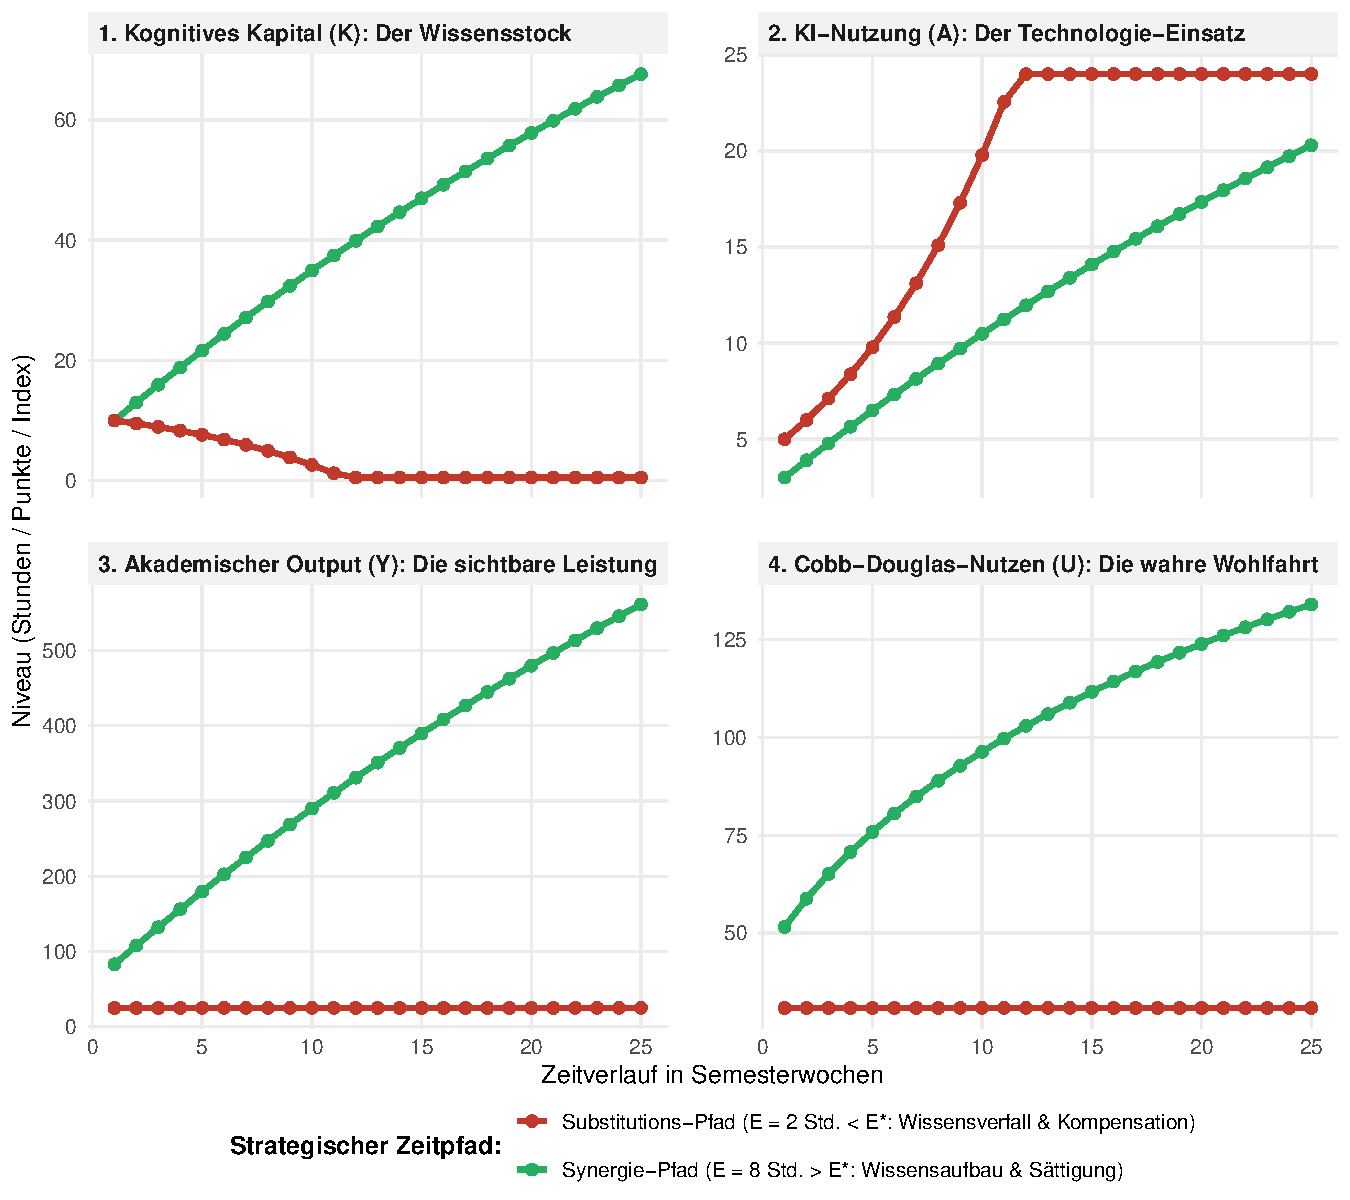
\includegraphics[keepaspectratio]{index_files/figure-pdf/fig-euler-paths-1.pdf}}

}

\caption{\label{fig-euler-paths}Intertemporale Dynamik der KI-Nutzung:
Synergie-Pfad vs.~Kompensations-Spirale}

\end{figure}%

\section{Fazit und hochschuldidaktische
Implikationen}\label{fazit-und-hochschuldidaktische-implikationen}

Das hier präsentierte Modell entzaubert zwei gängige Mythen: KI macht
Studierende weder automatisch produktiver, noch verleitet sie
zwangsläufig zur kognitiven Atrophie. Wie bei einem E-Bike entscheidet
die Intensität der eigenen Anstrengung (\(E_t\)) im Verhältnis zur
technologischen Schwelle (\(E^* = \frac{\gamma}{\beta}\)), in welche
Richtung das System kippt.Die hochschuldidaktische Brisanz dieses
Resultats offenbart sich beim Blick auf Panel 3 (Output) und Panel 4
(Nutzen) der Simulation:In einer rein ergebnisorientierten
Prüfungslandschaft fallen beide Studierendentypen kaum auseinander.
Student B erbringt durch die kompensatorische KI-Nutzung optisch
denselben akademischen Output wie zu Studienbeginn.Sein wahrer
Wohlfahrtsverlust zeigt sich jedoch im verborgenen Verfall seines
kognitiven Kapitals (Panel 1) und seinem stagnierenden Nutzen (Panel 4),
während Student A durch den Synergieeffekt eine massive
Wohlfahrtssteigerung und ein robustes Wissensplateau (\(K_{\max}\))
erreicht.Für die Gestaltung moderner Universitäten folgt daraus: Verbote
von KI-Systemen sind methodisch ebenso verfehlt wie das Verbot von
E-Bikes im Straßenverkehr. Stattdessen müssen Anreizstrukturen und
Prüfungsformate so neugestaltet werden, dass sie hohe eigene kognitive
Anstrengungen belohnen und erzwingen (\(E_t > E^*\)).Wird der
Eigenaufwand -- etwa durch mündliche Diskursprüfungen,
prozessbegleitendes Hinterfragen oder komplexe Problemlösungssettings --
zum unbedingten Komplement der KI-Nutzung gemacht, wirkt die Technologie
als intellektueller Hebel. Am Ende bewahrheitet sich auch im digitalen
Zeitalter eine alte Erkenntnis: De ingenio non est disputandum -- der
menschliche Verstand lässt sich nicht wegreformieren; er muss trainiert
werden.




\end{document}
